\documentclass[10 pt,usenames,dvipsnames, oneside]{article}
\usepackage{../../../modelo-ensino-medio}



\begin{document}

\begin{center}
  \begin{minipage}[l]{3cm}

\includegraphics[width=2cm]{logo}    
\end{minipage}\hfill
\begin{minipage}[r]{.8\textwidth}
 {\Large \scshape Atividade: Rede de Tráfego Rodoviários}  
\end{minipage}
\end{center}
\vspace{.2cm}

\ifdefined\prof
%Habilidades da BNCC
% \begin{objetivos}
% \item 
% \end{objetivos}

%Caixa do Para o Professor
\begin{goals}
%Objetivos específicos
\begin{enumerate}
\item Identificar um sistema linear com mais do que duas variáveis.
\item Resolver um sistema linear por escalonamento.
\end{enumerate}

\tcblower

%Orientações e sugestões
O objetivo dessa atividade é dar um primeiro exemplo de sistema linear escalonado. Apesar dele possuir 6 incógnitas, o formato desse tipo de sistema permite que a cada incógnita que tem seu valor determinado permite que se calcule o valor de uma outra incógnita do sistema. Assim, a solução do sistema é facilmente determinada.
\end{goals}

\bigskip
\begin{center}
{\large \scshape Atividade}
\end{center}
\fi

\begin{figure}[H]
\centering

\noindent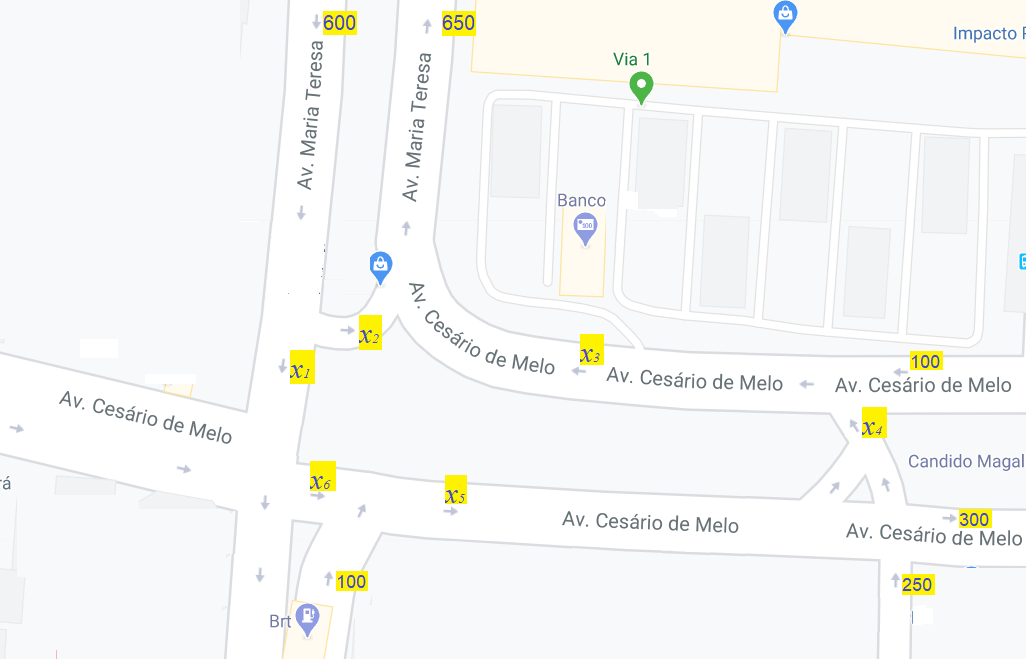
\includegraphics[width=375bp]{trafego.png}
\caption{Fonte: Adaptada do aplicativo Google Maps.}
\end{figure}

O mapa acima ilustra o trecho de uma rede rodoviária com grande movimento de carros em um bairro da cidade do Rio de Janeiro. Todas as avenidas destacadas no mapa são de mão única e as setas indicam o sentido em que os veículos trafegam sobre elas. Os valores destacados em amarelo em alguns trechos das avenidas representam o fluxo de veículos que passam por hora naquele trecho. Nessa rede de tráfego há conservação do fluxo de veículos, isto é, o fluxo de veículos que entra em uma bifurcação é igual ao fluxo de veículos que sai dessa bifurcação. Por exemplo, a figura mostra que por hora chegam $600$ veículos nesta rede através da Avenida Maria Teresa, sendo que na primeira bifurcação, uma certa quantidade $x_1$ de veículos continua em frente e outra quantidade $x_2$ entra pelo retorno da Avenida.  Pela conservação de fluxos temos:
$$
x_1 + x_2 = 600.
$$

\begin{enumerate}
\item{}
Com as informações que estão disponíveis no mapa e a conservação do fluxo de veículos, obtenha um sistema de equações envolvendo as incógnitas $x_1,x_2,..., x_6$.

\item{}
Suponha que um técnico da companhia de engenharia de tráfego aferiu que o valor da incógnita $x_6$ era de $400$ veículos por hora. Com essa informação e com o sistema obtido no item \titem{a)}, determine o valor das outras incógnitas destacadas no mapa. 

\item{}
O sistema que você obteve no item \titem{a)} tem mais de uma solução? Se sim, você consegue obter algumas?

\end{enumerate}

\ifdefined\prof
\begin{solucao}

\begin{enumerate}
\item 
$\left \{
\begin{aligned}
x_1+x_2&=600\\
x_2+x_3&=650\\
-x_3+x_4&=-100\\
-x_4+x_5&=50\\
-x_5+x_6&=100
\end{aligned}
\right.$
\item $(x_1,x_2,x_3,x_4,x_5,x_6)=(300,300,350,250,300,400)$
\item Sim. No item $b)$, ao atribuir o valor $400$ à incógnita  foi possível encontrar um valor para as demais incógnitas de forma que esses valores compunham uma solução para o sistema do item \titem{a)}. Atribuindo outros valores a $x_6$ e repetindo o processo realizado no item \titem{b)} pode-se obter infinitas soluções para este mesmo sistema.
\end{enumerate}

\end{solucao}
\fi

\end{document}